Для того, чтобы отдавать себе отчет в том что мы находимся на правильном пути, выбирая
модель для описания источника и щелевых устройств в схеме (раздел \ref{sec:source_section}, \ref{sec:slits_section}),
мы провели ряд экспериментов (рисунок \ref{ris:for_slits_scan}).

\begin{figure}[H]
  \centering
  \subfloat[]{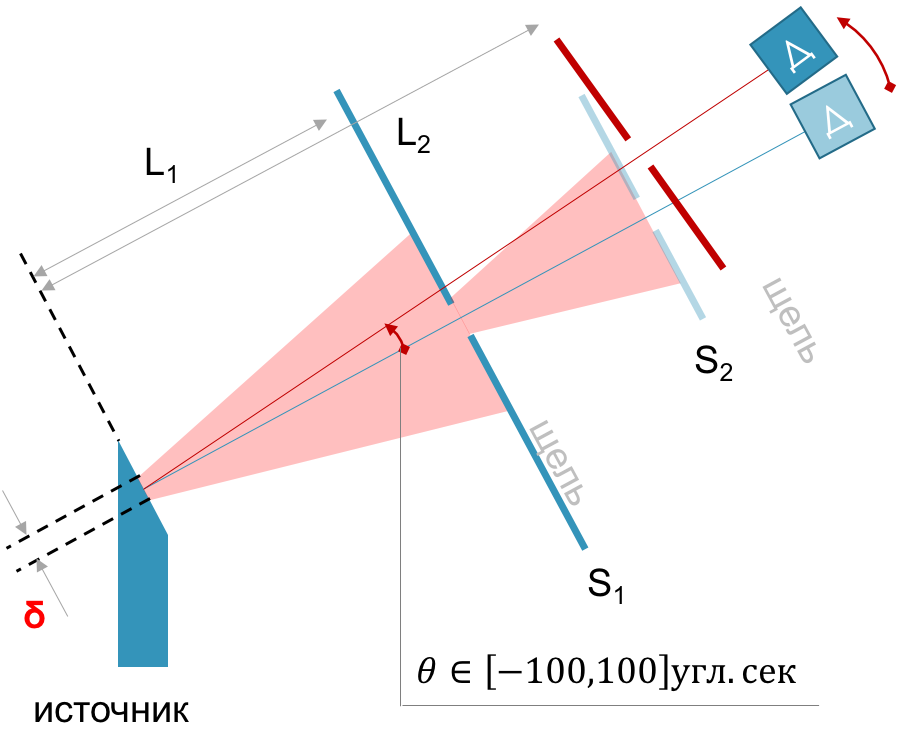
\includegraphics[width=0.52\textwidth]{images/for_slits_scan.png}}
  \hfill
  \subfloat[В случае точеного источника пределы интегрирования определяются из геометрического
   перекрывания щелевых устройств, в случае $\delta \neq 0$ - а и b увеличиваются и определяются из (\ref{sec:calc_slits_ability}).
  ]{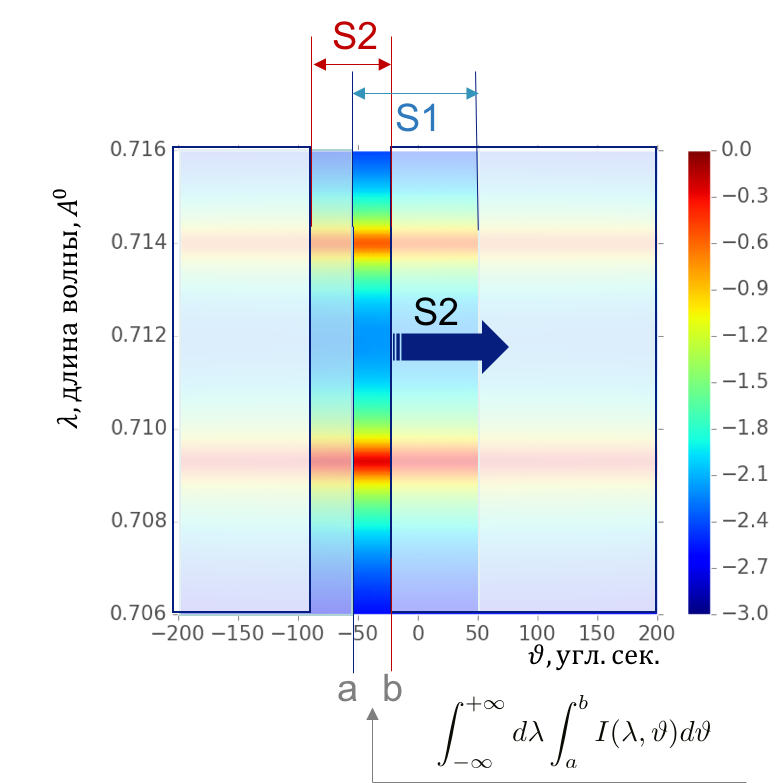
\includegraphics[width=0.45\textwidth]{images/for_slits_scan_int.png}}
  \caption{Схема эксперимента для апробации подхода к построению аппаратной функции дифрактометра}
  \label{ris:for_slits_scan}

\end{figure}
В виду отсутствия линейного детектора для прямого наблюдения углового распределения интенсивности рентгеновского
пучка после его прохождения через систему щелевых устройств (рисунок \ref{ris:calc_slits_ability_res}),
мы были вынуждены изменять угловое положение второго щелевого устройства (S2) и измерять суммарную интенсивность
за ним.

\begin{figure}[H]
  \centering
  \subfloat[$S_1 = 20$ мкм; $S_2 = 40$ мкм;]{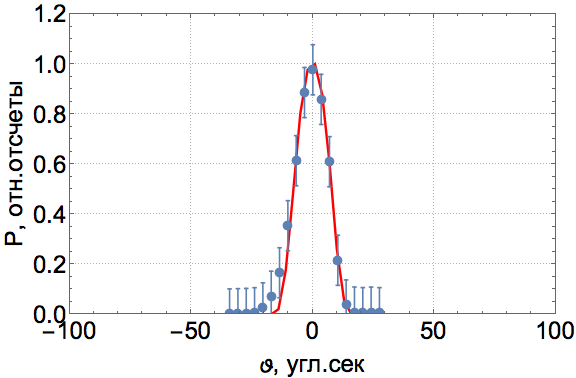
\includegraphics[width=0.3\textwidth]{images/zero_exp_20_40.png}}
  \hfill
  \subfloat[$S_1 = 40$ мкм; $S_2 = 40$ мкм;]{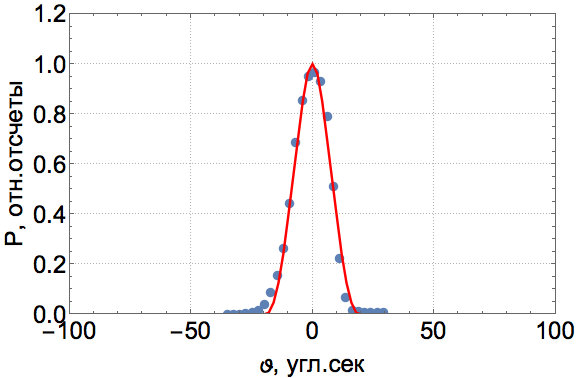
\includegraphics[width=0.3\textwidth]{images/zero_exp_40_40.png}}
  \hfill
  \subfloat[$S_1 = 50$ мкм; $S_2 = 100$ мкм;]{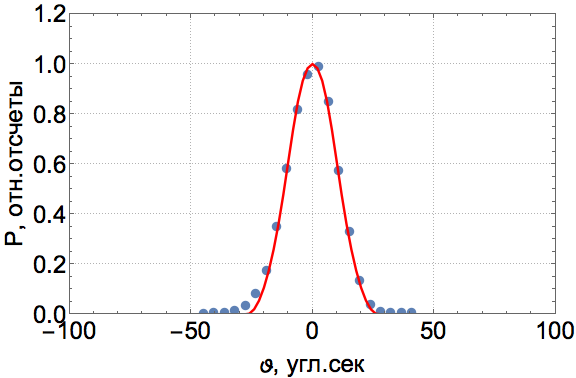
\includegraphics[width=0.3\textwidth]{images/zero_exp_50_100.png}}
  \hfill
  % \subfloat[$S_1 = 60$ мкм; $S_2 = 40$ мкм;]{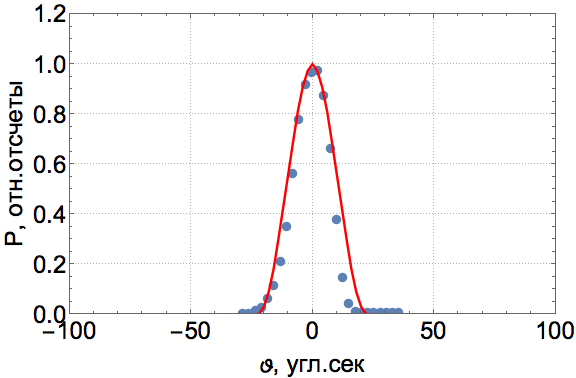
\includegraphics[width=0.3\textwidth]{images/zero_exp_60_40.png}}
  % \hfill
  \subfloat[$S_1 = 100$ мкм; $S_2 = 200$ мкм;]{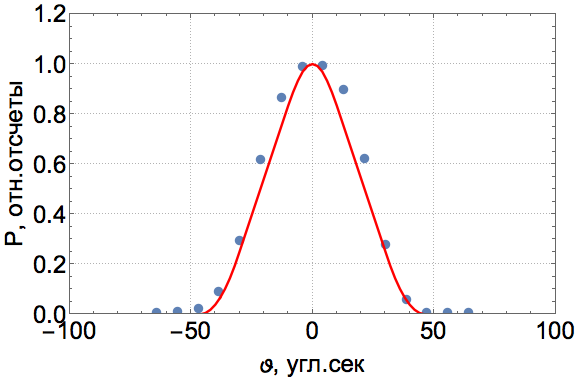
\includegraphics[width=0.3\textwidth]{images/zero_exp_100_200.png}}
  \hfill
  \subfloat[$S_1 = 100$ мкм; $S_2 = 300$ мкм;]{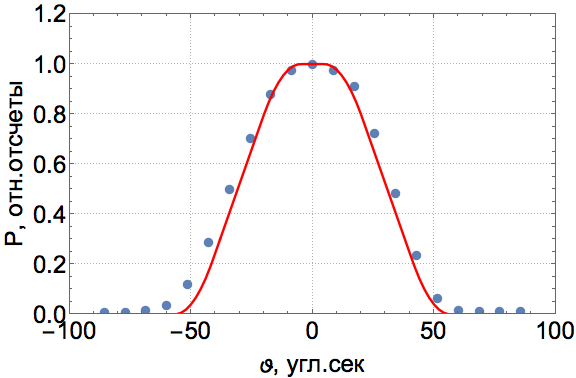
\includegraphics[width=0.3\textwidth]{images/zero_exp_100_300.png}}
  \hfill
  \subfloat[$S_1 = 200$ мкм; $S_2 = 20$ мкм;]{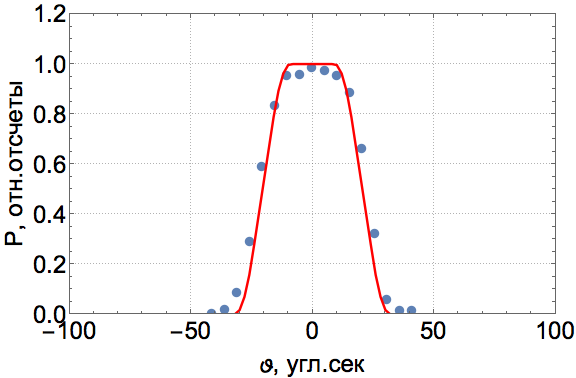
\includegraphics[width=0.3\textwidth]{images/zero_exp_200_20.png}}
  \hfill
  \subfloat[$S_1 = 200$ мкм; $S_2 = 200$ мкм;]{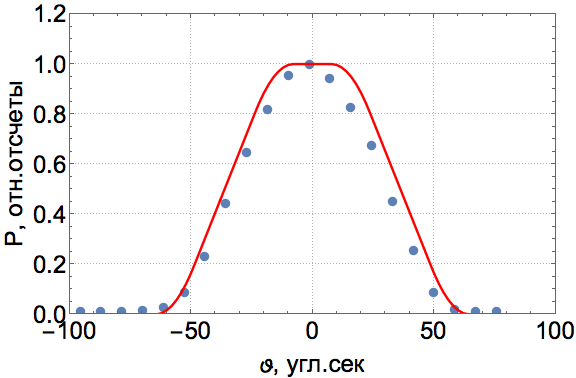
\includegraphics[width=0.3\textwidth]{images/zero_exp_200_200.png}}
  \hfill
  \subfloat[$S_1 = 200$ мкм; $S_2 = 300$ мкм;]{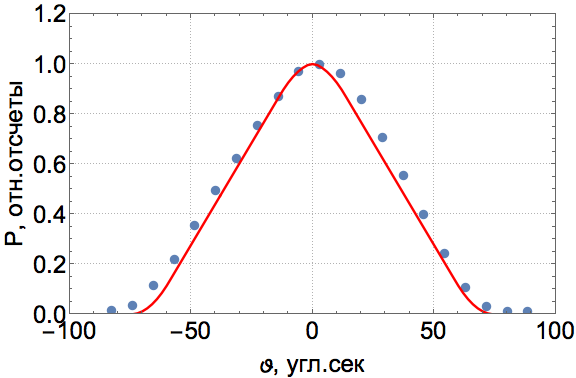
\includegraphics[width=0.3\textwidth]{images/zero_exp_200_300.png}}
  \hfill
  \subfloat[$S_1 = 300$ мкм; $S_2 = 300$ мкм;]{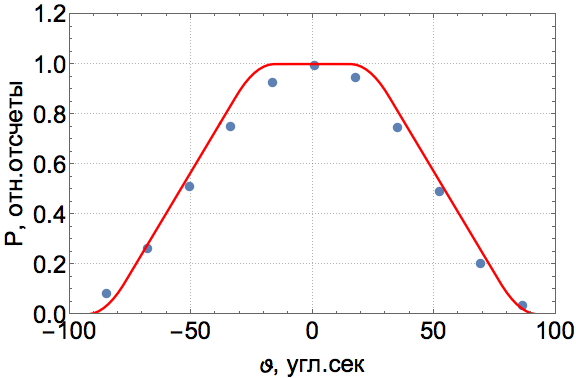
\includegraphics[width=0.3\textwidth]{images/zero_exp_300_300.png}}
  \caption{Нолькристальный эксперимент для разных размеров щелевых устройств; $L_1= 570 $мм,
  $L_2 = 1005$ мм; $\delta = 0.1$ мм; (красная линия) - расчет, (синие точки) - эксперимент.  }
  \label{ris:zero_exp}
\end{figure}
